\documentclass[11pt]{article}
\usepackage[T1]{fontenc}
 \usepackage{lmodern}
\usepackage[margin=1.02in]{geometry}
\usepackage{amsmath,amssymb,amsthm,mathtools}
\usepackage{microtype,booktabs,array}
\usepackage{tikz}
\usepackage[colorlinks=true,linkcolor=blue!50!black,citecolor=blue!50!black,urlcolor=blue!50!black]{hyperref}
\hypersetup{pdftitle={From Euclidean tensor prices to EPRL amplitudes: a rank obstruction at the 4-to-2 move}}

\newtheorem{theorem}{Theorem}[section]
\newtheorem{proposition}[theorem]{Proposition}
\newtheorem{lemma}[theorem]{Lemma}
\theoremstyle{remark}
\newtheorem{remark}[theorem]{Remark}
\DeclareMathOperator{\Inv}{Inv}
\DeclareMathOperator{\Sym}{Sym}
\DeclareMathOperator{\tr}{tr}
\DeclareMathOperator{\rank}{rank}
\DeclareMathOperator{\supp}{supp}
\DeclareMathOperator{\Span}{span}
\newcommand{\id}{\mathbf{1}}
\newcommand{\HH}{\mathcal H}
\newcommand{\J}{\mathbf J}
\newcommand{\pket}[1]{\lvert #1\rangle}
\newcommand{\pbra}[1]{\langle #1\rvert}
\newcommand{\braket}[2]{\langle #1 \mid #2 \rangle}
\newcommand{\proj}[1]{\pket{#1}\pbra{#1}}
\newcommand{\C}{\mathbb C}

\title{\textbf{From Euclidean tensor prices to EPRL amplitudes:}\\[2pt]
A rank obstruction at the four-to-two move}
\author{}
\date{26 November 2026}

\begin{document}
\maketitle
\begin{abstract}
A coherent valence-bond lift turns centrally smoothed Euclidean tensor prices into calibrated partial angular-momentum Casimirs on arbitrary finite \(\mathrm{SU}(2)\) intertwiner spaces. Their spectral projectors reconstruct the local operators of cutoff Euclidean EPRL spin foams. An oriented trace formula retains complex amplitudes and their internal-spin interference, and is compatible with standard Hilbert-space gluing for corrected edges. We then exhibit a finite obstruction to reducing the corrected four-to-two Pachner move to the old seam: with four base triangles fixed to spin zero, the two-simplex side factors through a one-dimensional intertwiner space, while a five-state submatrix of the four-simplex side is nonsingular. This holds for every rational \(0<\gamma<1\) and every nontrivial consecutive admissible-spin cutoff, with the minimal admissible spin used on the tagged boundary and the Spin(4) dimension used as face weight. The calculation rules out a scalar repair or a replacement of the two local vertex tensors that retains the same one-dimensional seam. It does not assert a continuum limit or derive the EPRL dynamics from the tensor spectrum.
\end{abstract}

\section{Introduction}

A Euclidean tensor price is an invariant of a tensor and a configuration of sites, not by itself a gravitational amplitude. The price theorem of OpenAI~\cite{OpenAI} nevertheless supplies a useful exact structure: a dimension-\(d\) wire between two sites costs their Euclidean separation times \(\log d\), and a compatible spectral point is additive under sitewise direct sum and multiplicative under sitewise tensor product. We use a specific coherent matching lift to turn this scalar information into quadratic forms on an intertwiner code. No geometric spacetime, dynamical coupling, or gauge constraint is inferred from the raw price. The code, the admissible spins, and the contractions are supplied independently.

The resulting operator dictionary lets one write the known local Euclidean EPRL construction~\cite{EPRL,Barrett} entirely in terms of calibrated cut projectors and oriented evaluation. In particular, the standard bare edge map is a product of simplicity and Haar projectors, while the corrected edge map is its support projector. The distinction is precisely the nonisometry and inverse-Gram correction already identified by Kami\'nski, Kisielowski and Lewandowski~\cite{KKL}. Likewise, oriented operator-foam gluing and its compatibility with edge subdivision are prior results~\cite{Operator}. Our contribution here is the coherent price representation: it computes these operators, preserves the amplitude phase under sewing, and supplies an exact finite Pachner calculation.

The main obstruction is stronger than unequal amplitudes for a pair of triangulations. We fix the common boundary base labels, choose five explicit states on each side of the boundary, and prove that the four-simplex kernel has rank five on that block. On the two-simplex triangulation the same block has rank at most one. Thus no adjustment of the two local vertices alone can work through the original seam. This is a specified corrected EPRL amplitude, not the holomorphic constrained model or a truncation of its loop identity studied by Banburski et al.~\cite{Holomorphic}. Nor is the result an alternative derivation of the nonlocal one-loop measure in linearized Regge calculus~\cite{Nonlocal}; it is an exact calculation on spin-network boundary states without a Regge saddle assumption.

Section~\ref{sec:dictionary} constructs the cut-price dictionary. Section~\ref{sec:foam} treats amplitudes and gluing. Sections~\ref{sec:pachner} and~\ref{sec:rank} contain the rank calculation. Throughout, logarithms are natural, group projectors use normalized Haar measure, and orientation is carried by the ordinary dual spaces.

\section{A spectral cut operator on intertwiner space}\label{sec:dictionary}

\subsection{Conditional price on a coherent code}

Fix placed sites of positive mean width \(W\), normalized so that a segment has its length. Let \(F\) be one compatible spectral point supplied by~\cite{OpenAI}, with price \(W\log F\). Consider a pure coded tensor
\[
 \Psi=\bigoplus_{i=1}^s \sqrt{p_i}\,\Psi_i,\qquad
 p_i\geq 0,\quad \sum_i p_i=1.
\]
The branch tensors have unit norm and their sectors are orthogonal at \emph{each} site; one classical label is coherently shared among the sites. Remove any zero-probability branch when using probabilities. Let \(f_i=F(\Psi_i)\). On \(r\) copies, make one coherent yes/no projection onto a set \(A\) of label words, without learning the successful label. The squared fidelity of the normalized success state is \(p^{\otimes r}(A)\). After this truncation its unlogged price is \(\sum_{\boldsymbol i\in A}\prod_{\ell=1}^r f_{i_\ell}\): spectral additivity and multiplicativity apply and the nonzero scalar coefficients in retained branches can be removed by an invertible map on one site's flag blocks.

Fix a discarded probability \(0<\epsilon<1\). The infimum, over these central postselections, of the price per copy converges to
\begin{equation}\label{eq:typ}
 W\left[H(p)+\sum_i p_i\log f_i\right],
 \qquad H(p)=-\sum_i p_i\log p_i.
\end{equation}
Indeed, set \(Y_i=\log(f_i/p_i)\). The weight of a word equals its probability times \(\exp(\sum_\ell Y_{i_\ell})\). With probability tending to one, the sample mean tends to \(\mathbb E_pY\). The typical set is feasible for large \(r\), bounding the rate from above. Any feasible set intersects the typical set in probability at least \(1-\epsilon-o(1)\), bounding the rate from below. This proves~\eqref{eq:typ}. No unrestricted approximate tensor conversion, or identification with one spectral point for all bipartite entropy functions, is presumed.

For Bell-wire branches, place one subset of sites close to \(0\) on a line and its complement close to \(1\), taking a limit through placements with distinct sites. The wire prices imply that the conditional part of~\eqref{eq:typ}, after subtracting the shared term \(WH(p)\), converges to the expected crossing wire price. All limits here apply to finite wire sums; no continuity claim is made for a general spectral point. Different cuts may use different placements on the same encoded space.

\subsection{The matching lift and the Casimir identity}

Let a node have legs of spins \(j_a\) with nonzero invariant space. Realize \(V_j=\Sym^{2j}(\C^2)\), and write \(2L=2\sum_a j_a\) for the number of constituent doublets. Let \(\HH_0=\Inv((\C^2)^{\otimes 2L})\) and \(J_S\) be the total angular momentum of a union \(S\) of physical legs; let \(u=\sum_{a\in S}2j_a\). If \(L=0\) all cut operators are zero. Otherwise, for each perfect matching \(M\) of the constituents, let \(v_M\) be the normalized product of spin singlets along \(M\). Its phase convention is immaterial to its projector. The isometry at the heart of the construction is
\begin{equation}\label{eq:lift}
 \mathcal V\psi=c_L^{-1/2}\sum_M
 \braket{v_M}{\psi}\,\pket{M}_{\mathrm{flags}}\otimes v_M,\qquad
 c_L=\frac{(2L-1)!!}{\mathrm{Cat}_L}.
\end{equation}
The same label \(M\) occurs at every physical site. By Schur--Weyl duality the spin-zero subspace is an irreducible permutation-group representation of dimension \(\mathrm{Cat}_L=(2L)!/[L!(L+1)!]\)~\cite{FH}. The matching projector sum commutes with all constituent permutations; its trace gives \(c_L\id\). This proves that~\eqref{eq:lift} is isometric, including on the physical symmetric-leg subspace. The enlarged branch vectors need not individually be symmetric within each original leg; symmetrization specifies the \emph{input} code.

\begin{theorem}[Conditional cut price]\label{thm:casimir}
For the lift~\eqref{eq:lift}, the conditional cut price is the expectation of the self-adjoint operator
\begin{equation}\label{eq:casimir}
 A_S=(\log 2)\left[
 \frac{u(2L-u)}{2(L+1)}\id+
 \frac{2}{L+1}\frac{\J_S^2}{\hbar^2}\right].
\end{equation}
It follows that spectral projectors onto any prescribed subset spin can be evaluated as polynomials in \(A_S\) on the same finite intertwiner space.
\end{theorem}

\begin{proof}
In a matching branch the cut crosses \(N_S(M)\) dimension-two wires, so \eqref{eq:typ} with the shared entropy removed gives the quadratic form of \((\log2)\mathcal V^\dagger\operatorname{diag}(N_S)\mathcal V\). The branch projectors for matchings containing a specific pair \(x,y\) sum to \(c_{L-1}P^-_{xy}\) on \(\HH_0\), where \(P^-_{xy}\) projects onto that pair's singlet. This follows by factoring off the pair and summing the remaining matchings; its complement is automatically a total singlet if the state on the pair is one. With \(c_0=1\), the ratio \(c_{L-1}/c_L=2/(L+1)\). Now \(N_S=u-2\sum_{x<y\in S}\id_{\{xy\in M\}}\). Since \(P^-_{xy}=\id/4-\J_x\cdot\J_y/\hbar^2\), summing it over pairs internal to \(S\) gives \(u(u+2)\id/8-\J_S^2/(2\hbar^2)\). Substitution yields \eqref{eq:casimir}, and the Casimir for a union of full legs commutes with their symmetrization. Polynomial interpolation on its finite spectrum gives the projections.
\end{proof}

In particular \([\J_{ab}^2,\J_{ac}^2]=4i\hbar\,\J_a\cdot(\J_b\times\J_c)\), so the noncommuting compressed operators recover the oriented triple-flux factors of the usual quantum polyhedron volume~\cite{Barbieri,BianchiHaggard}:
\[
 \J_a\cdot(\J_b\times\J_c)
 =\frac{(L+1)^2\hbar^3}{16i(\log2)^2}[A_{\{a,b\}},A_{\{a,c\}}].
\]
This is an operator statement on one common code, not a claim that scalar prices in one unknown state determine its oriented volume. Valence-bond crossing counts and flux commutators are not invented here; the connection is their identification in the coherently lifted, centrally smoothed Euclidean price. In particular the branch multiplication and direct sums in this lift matter~\cite{Alet}.



\paragraph{Why exact scalar prices alone do not suffice.}
On a fixed matching lift, any two states with the same nonzero matching support are related by a diagonal invertible map on one site's flags: the diagonal entry is the ratio of their branch amplitudes. Monotonicity in both directions makes \emph{every} exact spectral point agree on those lifted states, even before selecting a particular price. In the two-dimensional singlet space of four spin halves choose a real orthonormal pair \(u,v\). The states \((u+iv)/\sqrt 2\) and \((u-iv)/\sqrt 2\) have full matching support because the matching vectors can be chosen real. Their oriented triple-flux expectations are nonzero and opposite: in that real basis the commutator of the two distinct real pair Casimirs is a nonzero real antisymmetric matrix, and the displayed triple flux is its imaginary multiple. Even their scalar matching probabilities agree. Thus recovering the oriented operator requires the coherent code and its quadratic forms across inputs (or equivalent phase-sensitive operator access). It is not a reconstruction from the list of exact scalar prices of a single state.


\section{Cut projections and coherent spin-foam gluing}\label{sec:foam}

\subsection{The edge operator}

We consider \(0<\gamma<1\). For each admissible physical face spin \(k\) the two chiral labels are \(j^\pm=(1\pm\gamma)k/2\). They are half-integral, and the selection is the maximum total diagonal spin \(k=j^++j^-\). The following local operator expressions also make sense with a different selected chiral pair spin, but our rank theorem will use this maximum branch.

At an edge end let \(W_e\) be the product of the incident chiral factors, oriented as spaces or duals. Let \(M_e\) be the product of projectors that select total diagonal \(k\) on each face pair \(V_{j^+}\otimes V_{j^-}\). Let \(G_e\) project separately onto the total plus and minus singlets. On the common diagonal-singlet space these projectors are supplied by Theorem~\ref{thm:casimir}. Let \(Y_e\) be the product of normalized Clebsch inclusions, initially restricted to the invariant physical intertwiner space, and \(B_e=G_eY_e\) the usual EPRL map. Its bare and corrected chiral edge operators are
\begin{equation}\label{eq:Q}
 Q_e=B_eB_e^\dagger=G_eM_eG_e,\qquad
 P_e=\supp Q_e=B_e(B_e^\dagger B_e)^+B_e^\dagger ,
\end{equation}
where \(+\) means the Moore--Penrose inverse. For the second equality defining \(Q_e\), the product Clebsch inclusion on the full incoming tensor product has range \(M_e\), and \(G_e\) already enforces the diagonal invariant. Thus restricting the incoming factors to a diagonal singlet makes no difference to \(Q_e\). The operator \(P_e\) is the orthogonal projector onto the EPRL image, i.e.\ the corrected construction of~\cite{KKL,Operator}. It can be computed by polynomial interpolation on \(Q_e\) (zero at \(0\) and one on its positive eigenvalues). It is not in general the projector onto the simultaneous intersection of the two ranges \(G_e\) and \(M_e\). No arbitrary inverse-Gram matrix is needed once orthogonal image gluing has been specified.

\subsection{A signed trace at fixed spins}

Take a finite oriented closed foam and a fixed coloring, with \(H\) the common diagonal-singlet space of the full set of chiral edge-end factors. At an oriented pair of equal-spin dual factors use the normalized Hilbert cup \(d^{-1/2}\sum_\alpha\pket{\alpha}\otimes\pket{\bar\alpha}\). Write \(\Xi\) for the product of cups across the two ends of each edge strand and \(\Omega\) for the product of cups at vertex wedges. These are separate perfect pairings, both in \(H\). Let \(E\) be the product of edge operators, placed at one end of each edge-end pairing with the corresponding transpose on the dual side when the placement is switched. Thus vectorization gives the normalized fixed-spin contraction \(z=\pbra{\Omega}E\pket{\Xi}\). All singlet pair effects defining \(\Pi_\Xi=\proj{\Xi}\) and \(\Pi_\Omega=\proj{\Omega}\) are recovered from Theorem~\ref{thm:casimir}, with one common lift on \(H\).

The alternating cycles of the two pairings give a known, nonzero kinematic overlap \(s=\braket{\Xi}{\Omega}\). A chiral cycle with \(r\) pairs of each type contributes \(d^{1-r}\): there are \(2r\) factors of \(d^{-1/2}\) and a single free magnetic trace of dimension \(d\). In particular a one-pair cycle gives one. Thus
\begin{equation}\label{eq:trace}
 z=\frac{\tr_H(\Pi_\Xi\Pi_\Omega E)}{s}.
\end{equation}
The numerator, unlike the individual expectation of a rank-one effect, retains its orientation-dependent phase. Equation~\eqref{eq:trace} is the rank-one identity for \(\tr_H(\proj{\Xi}\proj{\Omega}E)\); the phase reference is an elementary wire loop count, not an input gravitational amplitude. Orientations and dualities are fixed for all spin sectors alike. In a self-dual magnetic basis, changes of cup convention would have to carry their corresponding signs; we use oriented \(V\)-\(V^*\) evaluation throughout.

At a fixed matrix element of an open foam, let \(\Xi_b\) consist of internal edge cups and the supplied oriented chiral boundary tensors. For the kinematic reference \(\Xi_{\rm ref}\), replace the boundary tensors by normalized pairings of the endpoints of the exterior face arcs. The resulting two pairings close into alternating cycles just as above. The formula is
\begin{equation}\label{eq:open-trace}
 \pbra{\Omega}E\pket{\Xi_b}
 =\frac{\tr_H(\pket{\Xi_b}\pbra{\Xi_{\rm ref}}\Pi_\Omega E)}
             {\braket{\Xi_{\rm ref}}{\Omega}}.
\end{equation}
The boundary phase is supplied by the actual boundary tensor, not by a single positive effect. The reference does not need to be a physical EPRL state. To return to the ordinary unnormalized oriented cup and cap convention, multiply by \(\sqrt d\) for each actual normalized map that was replaced (not for the auxiliary reference). Face weights are then applied in the declared model convention. At a finite cutoff the state sum adds the resulting complex scalars, not their squares, before any modulus is taken.

\subsection{Composition}

For a fixed cutoff and a boundary graph \(\Gamma\), use the direct sum over common link labels of the tensor products of the supported edge-end spaces \(K_e=\operatorname{ran}P_e\) at the boundary vertices. Give these the induced Hilbert metrics. If conventional physical intertwiner vectors are desired, use the supported domain \(\ker(B_e)^\perp\) and its polar isometry \(U_e=B_e(B_e^\dagger B_e)^{+1/2}\) onto \(K_e\). This choice does not presume injectivity in a sector with a missing target. An incoming boundary uses the inclusion of \(K_e\), and its outgoing partner uses the adjoint (or \(U_e,U_e^\dagger\) in the physical basis). At an internal edge use \(P_e\).

For definiteness, consider oriented collared diagrams in which the gluing loci on each face are disjoint proper arcs, including their endpoints. If a connected face surface \(F\) has \(b(F)\) boundary arcs and a positive label weight \(w(k)\), assign the factor \(w(k)^{\chi(F)-b(F)/2}\). An internal disk carries \(w(k)\), a disk meeting one boundary arc carries \(\sqrt{w(k)}\), and an identity strip carries one. Under sewing along \(h\) disjoint arcs, the Euler characteristic decreases by \(h\) and \(b\) decreases by \(2h\); the exponent is additive, also for identifications of disjoint arcs on a formerly connected face. One may restrict to sewings that preserve ordinary disk faces; this weight states precisely the convention used if regular face surfaces of more general topology are included.

\begin{proposition}[Finite compositional evaluation]\label{prop:glue}
At matched cutoffs, orientations and face weights, the corrected amplitudes compose by ordinary Hilbert-space contraction, preserve disjoint union, and send reversal with adjointed decorations to the adjoint. The identity cylinder is the identity on the supported boundary space.
\end{proposition}
\begin{proof}
Expand a sewing in an orthonormal basis of the common boundary Hilbert space. The spin sums identify the labels on all shared face arcs; piecewise equalities on a face give exactly its eventual single color, with no extra multiplicity. On every common boundary vertex the intertwiner sum inserts the chiral projector \(P_e\), from inclusion followed by its adjoint. This is the required corrected edge. The unnormalized dual cups and caps have the exact snake relation, and the face scalars multiply by the preceding Euler identity. Thus this contraction is exactly the amplitude of the sewn foam. The same identities evaluate an identity cylinder, and \(P_e^2=P_e\) allows transparent subdivisions of a corrected edge. Disjoint vertex/edge sums factor under disjoint union, and reversing the orientation exchanges cups/caps and all indicated adjoints. Equations~\eqref{eq:trace} and~\eqref{eq:open-trace} evaluate those same complex amplitudes, so the price representation preserves the sewing rule.
\end{proof}

This is the familiar operator-foam sewing~\cite{Operator} expressed using coherent cut operators, not invariance under the insertion of additional curvature-bearing simplices. Inserting the bare \(B_e\) on both sides of an unweighted physical boundary resolution would give \(Q_e\) rather than \(P_e\) and generally would not define a transparent subdivision. The bare model is instead retained on marked diagrams by inserting one \(Q_e|_{K_e}\) coupon per original edge (or two prescribed \(\sqrt{Q_e}|_{K_e}\) halves). This distinction is about the edge Hilbert metric, not the phase anchor.

\section{The four-to-two block at fixed cutoff}\label{sec:pachner}

\subsection{Triangulations and boundary states}

Let the six ball vertices be \(A,B\) and \(W=\{1,2,3,4\}\). The four triangulation simplices are \(AB(W\setminus\{i\})\) for \(i\in W\); the two are \(AW,BW\). Their exterior tetrahedra are the same, namely \(A(W\setminus\{i\})\) and \(B(W\setminus\{i\})\). Fix all four exterior triangles lying in \(W\) to spin zero. On the two side these also determine the complete coloring of the connecting tetrahedron \(W\), whose corrected intertwiner space is one-dimensional. For every allowed choice of external states at the two tips, the two-side matrix therefore factors through \(\C\). Modifying either vertex or multiplying the entire amplitude by a scalar cannot increase that intermediate dimension.

For rational \(0<\gamma<1\), let \(s>0\) be the smallest admissible nonzero physical spin. The two numbers \(2j_s^\pm=(1\pm\gamma)s\) are positive integers. The half-integrality constraints on the scaled physical spin define an integer lattice, so the set of nonnegative admissible spins is \(\{ms:m\in\mathbb{N}_0\}\). At least one of \(j_s^\pm\) is strictly half-integral: if both were integers, then \(s=j_s^++j_s^-\) would be an integer and \(s/2\) another positive admissible label. Use the consecutive cutoff \(m=0,\dots,N\), \(N\geq1\), the projector \(P_e\) at each corrected edge, and face weights
\begin{equation}\label{eq:D}
 D_m=(2m j_s^++1)(2m j_s^-+1),\quad
 D=D_1,\quad
 V_N=\sum_{m=0}^N D_m^2,\quad
 S_r=\sum_{m=0}^{N-r}D_mD_{m+r}.
\end{equation}
Empty sums vanish. When shifted, set \(D_m=0\) outside the cutoff.

On each tip choose vacuum and four \emph{tags}, indexed by \(i\in W\). The tag \(i\) at tip \(A\) places spin \(s\) on the three boundary triangles \(Aij\) for \(j\ne i\); the corresponding tag at \(B\) uses \(Bij\). All other triangle labels at that tip are zero. Each affected boundary tetrahedron is bivalent after trivial factors are removed; use its normalized supported singlet tensor. Equivalently, the three boundary links form a normalized Wilson-character triangle. In particular, cycling the three unmarked outer vertices fixes the tag state with no choice of an additional sign. The orientation-preserving group \(A_4\) acts transitively on tags and on ordered unequal tag pairs. The foam and these boundary tensors are equivariant, so the four-side tag block has a constant diagonal and a constant off-diagonal, and the vacuum--tag entries do not depend on the choice of tag. No odd renaming of the simplices is needed for this symmetry.

We strip off the common nonzero, boundary-only face factors. We then multiply each tag row and column by \(D^{1/2}\), the reciprocal of its two-side triangle amplitude, and divide the four-side amplitude by \(V_N\). All these scalings are invertible and do not change rank. We shall prove that the resulting block has the form
\begin{equation}\label{eq:block}
 \begin{pmatrix}
 1 & c\mathbf{1}^{\mathsf T}\\
 c\mathbf{1} & (a-b)I_4+b\,\mathbf{1}\mathbf{1}^{\mathsf T}
 \end{pmatrix},
 \qquad \mathbf{1}=(1,1,1,1)^{\mathsf T},
\end{equation}
with explicit formulas below.


\begin{figure}[tb]
\centering
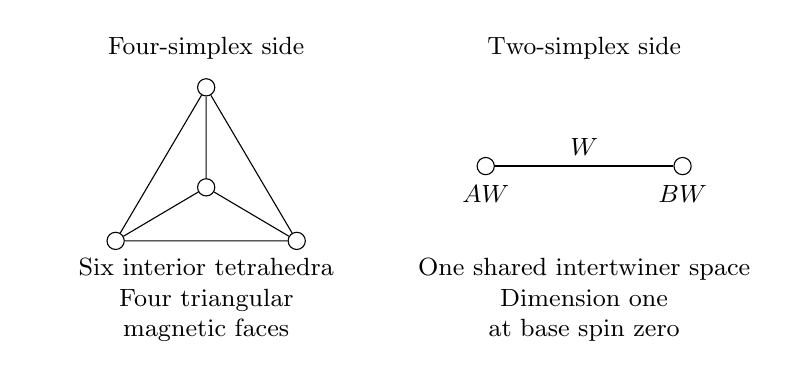
\begin{tikzpicture}[x=1cm,y=1cm,every node/.style={font=\small}]
 \node at (0,1.55) {Four-simplex side};
 \node[circle,draw,inner sep=2.2pt] (a) at (-1.15,-.9) {};
 \node[circle,draw,inner sep=2.2pt] (b) at (1.15,-.9) {};
 \node[circle,draw,inner sep=2.2pt] (c) at (0,1.05) {};
 \node[circle,draw,inner sep=2.2pt] (d) at (0,-.22) {};
 \draw (a)--(b)--(c)--(a) (d)--(a) (d)--(b) (d)--(c);
 \node[text width=4.3cm,align=center] at (0,-1.65)
   {Six interior tetrahedra\\Four triangular magnetic faces};
 \node at (4.8,1.55) {Two-simplex side};
 \node[circle,draw,inner sep=2.2pt,label=below:{$AW$}] (l) at (3.55,.05) {};
 \node[circle,draw,inner sep=2.2pt,label=below:{$BW$}] (r) at (6.05,.05) {};
 \draw[thick] (l)--node[above]{$W$}(r);
 \node[text width=4.3cm,align=center] at (4.8,-1.65)
   {One shared intertwiner space\\Dimension one at base spin zero};
\end{tikzpicture}
\caption{The interior dual graphs. On the four side the four magnetic faces form the boundary of a tetrahedron in the dual incidence structure. Boundary links and the tag labels are omitted.}
\label{fig:duals}
\end{figure}

\subsection{Closed strands and the vacuum}

At a normalized chiral bivalent invariant, the identification of the two oriented strands is \(d^{-1/2}\) times the ordinary identity wire. A \(q\)-cycle of these invariants in one chirality therefore has value \(d^{1-q/2}\). This follows by counting one free index trace and \(q\) normalization factors. Multiplying the two chiral contributions replaces \(d\) by \(D_m\) at spin \(ms\).

For vacuum at both tips, the interior triangles \(ABi\) are the only possibly nonzero labels. Each of the six interior tetrahedra \(ABij\) has two such labels and two zero labels. Its bivalent invariant enforces equality of its two labels, hence one common \(m\). Its corrected edge is the rank-one projector onto the product of the normalized chiral singlets. The magnetic faces form the oriented tetrahedral sphere in Figure~\ref{fig:duals}; orient it coherently. The active three-cycle at each simplex contributes \(D_m^{-1/2}\), the four faces yield \(D_m^4\), and the fixed-label amplitude is \(D_m^2\). Its sum is \(V_N\), as used in \eqref{eq:block}. The two-side vacuum is one.

For comparison the bare bivalent operator is \(Q_e=(2ms+1)P_e/D_m\). The scalar is the squared overlap of the normalized diagonal-spin cup with the normalized product chiral cup: the latter is a maximally entangled vector on dimension \(D_m\) and gives weight \((2ms+1)/D_m\) to the selected subrepresentation. With that different edge convention one obtains the vacuum sum \(\sum_m D_m^2[(2ms+1)/D_m]^6\), not \(V_N\). Thus the corrected choice plays a substantive role.

\subsection{Same tag and single tag}

Fix a tag \(i\) and denote the label index on \(ABi\) by \(n\), and that on the three other interior triangles by \(m\). The latter must be equal by the bivalent edges whose outer vertices do not include \(i\). Orient each tag's boundary face fan along with its face \(ABi\) as a disk, with \(ABi\) oriented as in the internal sphere. At every touched interior tetrahedron the tag leg and \(ABi\) are then dual orientations. This convention fixes the positive normalized oriented contractions used below; it does not rely on arbitrary separate vertex phases.

With the same tag at both tips, the half-integral chirality forces \(n+m\) even and the polygon condition forces \(|n-m|\leq2\). The three interior tetrahedra touching \(ABi\) have the same four-valent edge projector \(P_{n,m}\) in the role order \(n,m,\mathrm{top},\mathrm{bottom}\). In each of the three simplices containing \(i\), the \(n\) leg pairs directly; the \(m\) leg and the two tag legs pass through one normalized bivalent transport each. Up to the factor \(D_m^{-1/2}D^{-1}\), this is the canonical pairing of the identical ordered four-leg spaces. Sewing around \(ABi\) gives \(\tr(P_{n,m}^3)=\rank P_{n,m}\). The simplex omitting \(i\) contributes \(D_m^{-1/2}\). Thus the four interior face factors \(D_nD_m^3\) yield the usual weighted coefficient \(D_nD_m\rank P_{n,m}/D^3\) before the boundary rescalings.

Write \(r_0=2s+1\). The ranks are \(r_0\) for \(n=m\ge1\), one at \(n=m=0\), and one for \(|n-m|=2\) within the cutoff. To see this, couple the two tag legs to a physical spin. For \(n=m\ge1\) every spin from \(0\) to \(2s\) is allowed; for \(n=m=0\) only \(0\) is possible; and for \(|n-m|=2\) only \(2s\) is possible. The two chiral invariant spaces are nonzero by their polygon and parity conditions in these cases. We use EPRL injectivity into a nonzero target for the rational maximum branch, as proved by Kami\'nski, Kisielowski and Lewandowski~\cite{Injectivity}. Therefore
\begin{equation}\label{eq:a}
 a=\frac{A_N}{D^2V_N},\qquad
 A_N=r_0V_N-(r_0-1)+2S_2 .
\end{equation}

For one tag and vacuum, \(n+m+1\) must be even and \(|n-m|\le1\), hence \(n=m\pm1\). At each simplex containing \(i\), two normalized trivalent tensors pair along the \(n\) leg and through one bivalent transport on each of the \(m\) and tag legs. Both latter legs are opposite to \(n\) in orientation at each of those tetrahedra; the two tensors are literal duals in the same role order, so the contraction is positive and equals \(D_m^{-1/2}D^{-1/2}\). The other simplex gives \(D_m^{-1/2}\). The trivalent invariants exist on the saturated triangle supports, and their EPRL maps are nonzero by the same injectivity result. Including \(D_nD_m^3\) gives \(D_nD_m/D^{3/2}\) before rescaling each single-tag amplitude by \(D^{1/2}\). Thus
\begin{equation}\label{eq:c}
 c=\frac{2S_1}{D V_N}.
\end{equation}

\subsection{Unequal tags: oriented crossed contraction}

Let \(i\) be the top tag and \(j\ne i\) the bottom tag. Use \(n,p\) for the indices on \(ABi,ABj\); the other two outer vertices \(k,l\) have one common index \(m\) by the bivalent tetrahedron \(ABkl\). At the four trivalent tetrahedra \(ABik,ABil,ABjk,ABjl\) the independent chiral triangle and half-integral chirality rules force
\[
 n,p\in \{m-1,m+1\}\cap[0,N].
\]
There are two simplices containing both \(i,j\). At each of them the two trivalent tensors join along their \(m\) factors, with a separate bivalent transport on each tag strand. The tensor obtained by contracting their \(m\) factors has norm \(D_m^{-1/2}\): each normalized trivalent tensor is an isometry out of the \(m\) factor scaled by \(D_m^{-1/2}\), and the contraction of the two maps sums \(D_m\) mutually orthogonal terms. The two tag transports multiply by \(D^{-1}\). Thus the resulting four-leg tensor at \(ABij\) is a unit tensor \(u_{n,p;m}\) times \(D_m^{-1/2}D^{-1}\); its normalized pairings couple \((n,s)\) and \((p,s)\) through the intermediate \(ms\) in the separate chiralities, with \(n,p\) here denoting the spin indices.

To check the phase, orient the interior sphere and both tag disks as above. At \(ABij\) the \(n\) and \(p\) factors have opposite orientations, and the top and bottom tag factors are respectively opposite to \(n\) and \(p\). At \(ABik,ABil\) the \(m\) and top strands are both opposite to \(n\); at \(ABjk,ABjl\) the \(m\) and bottom strands are both opposite to \(p\). Hence the joined \(m\) factors in each of the two simplices are dual, and both ordered four-leg tensors at the ends of \(ABij\) are literal oriented duals: every role is reversed when passing to the other end. This edge consequently gives
\[
 q_{n,p;m}=\pbra{u_{n,p;m}}P_{n,p}\pket{u_{n,p;m}}\in[0,1].
\]
The two other simplices each pair two role-matched normalized trivalent tensors and supply \(D_m^{-1/2}D^{-1/2}\), including the same positive dual pairing as in the single-tag case. Combining these factors with \(D_nD_pD_m^2\) and the boundary rescalings proves
\begin{equation}\label{eq:b}
 b=\frac{1}{D^2V_N}\sum_{m=0}^N
 \sum_{n,p\in\{m-1,m+1\}\cap[0,N]}D_nD_p\,q_{n,p;m}.
\end{equation}
The essential point is that this is an oriented projector matrix element, not a product of separate modulus-squared vertex weights.

\section{The five-dimensional rank obstruction}\label{sec:rank}

\subsection{Three exact crossed weights and one lower bound}

For \(n=p=m-1\), the physical pair \((ns,s)\) is coupled at its maximum. In the maximal EPRL branch it maps only to the pair of chiral maxima: any smaller chiral spin would have too small a sum to contain that physical channel. Consequently \(u_{n,p;m}\) belongs to the EPRL image and \(q=1\). For \(n\ne p\) the two physical paired ranges meet at a single extremal intermediate spin, and so do the two paired ranges in each chirality. The nonzero corrected image is the entire resulting chiral line, so \(q=1\) here too. Only \(n=p=m+1\), in which the selected intermediate spin is minimal in both chiralities, need not give one.

In the exceptional case \(\gamma=1/3\), where \(s=3/2\) and \(r_0=4\), we will need the uniform estimate
\begin{equation}\label{eq:qbound}
 q_m:=q_{m+1,m+1;m}\geq
 \frac{t_m^2}{t_m^2+(1-t_m)^2}\geq\frac45,\qquad
 t_m=\frac{(3m+4)(2m+1)(m+1)}{(3m+1)(2m+3)(m+2)} .
\end{equation}
We give an analytic proof, including the normalizations.

In the Bargmann realization the highest vector of the minimal spin \(J-s\) in \(V_J\otimes V_s\), for \(J\ge s\), is proportional to the polynomial \([u,v]^{2s}u_1^{2(J-s)}\), with \([u,v]=u_1v_2-u_2v_1\). Its squared norm is
\[
 (2s)!(2J)!\frac{2J+1}{2J-2s+1}.
\]
Indeed, expanding the bracket and using the monomial factorial norm reduces the ratio to \(\sum_{r=0}^{2s}\binom{2s}{r}/\binom{2J}{r}=(2J+1)/(2J-2s+1)\). The latter follows by integrating \(x^r(1-x)^{2J-r}\) and summing with the binomial theorem. The adjoint of the norm-preserving maximal chiral Clebsch embedding is polynomial multiplication, with coefficient \(\sqrt{(2J_+)!(2J_-)!/(2J)!}\) at the large leg and its counterpart at the small leg. Multiplying the minimum highest-weight polynomials for \(J_+=m+1,J_-=(m+1)/2\) and \(s_+=1,s_-=1/2\) gives exactly the physical minimum highest-weight polynomial for \(J=3(m+1)/2,s=3/2\). Their norm ratio is the squared pair recoupling coefficient \(t_m\) in \eqref{eq:qbound}. Cross multiplication gives \(t_m\ge2/3\) since \(m(6m^2+5m-5)\ge0\) for integers \(m\ge0\); also \(t_m\to1\).

In the EPRL column originating from the minimum physical pair spin \(l\), the modulus of a row \((p',q')\) equals the squared pair recoupling modulus times \(\sqrt{(2l+1)/[(2p'+1)(2q'+1)]}\). This is the overlap between normalized vectorizations of the pair projector and its two chiral identities, giving one trace of dimension \(2l+1\). The two pair dimensions of the minimal row are the smallest denominators. The squared pair recoupling coefficients in all other rows sum to \(1-t_m\), since the chiral coupled pair basis is orthonormal. Projecting onto this single EPRL column already gives a lower bound on projection onto the full EPRL image. Bounding its squared norm with the minimal row denominator and using \(\sum_{i\ne0}|c_i|^4\leq(1-t_m)^2\) proves \eqref{eq:qbound}. The same estimate also yields \(q_m\to1\).

\subsection{Finite positive gaps}

Let
\begin{equation}\label{eq:B}
 B_N=\sum_{m=0}^N(D_{m-1}+D_{m+1})^2
     =2V_N-1-D_N^2+2S_2 .
\end{equation}
The possibly deficient weights \(n=p=m+1\) sum, before their \(q\)'s, to \(V_N-1\). In view of \eqref{eq:b},
\[
 \frac{B_N-\delta(V_N-1)}{D^2V_N}
 \le b\le \frac{B_N}{D^2V_N},
 \quad
 \delta=\begin{cases}
 1/5,&\gamma=1/3,\\
 1,&\text{otherwise}.
 \end{cases}
\]
Only the exceptional case uses the nontrivial bound \eqref{eq:qbound}.

\begin{theorem}[Rank five at every cutoff]\label{thm:rank}
For every rational \(0<\gamma<1\) and each \(N\ge1\), the five-state block \eqref{eq:block} of the corrected four-simplex amplitude has rank five. The two-simplex amplitude on the same boundary factors through a one-dimensional seam and has rank at most one.
\end{theorem}
\begin{proof}
On the three-dimensional tag-difference space the eigenvalue is \(a-b\), and
\[
 D^2(a-b)\ge
 \frac{(r_0-2)(V_N-1)+D_N^2}{V_N}>0.
\]
The remaining block, in the basis of vacuum and the unit uniform tag, is
\(\begin{psmallmatrix}1&2c\\2c&a+3b\end{psmallmatrix}\). Since
\(2S_1=\sum_mD_m(D_{m-1}+D_{m+1})\), Cauchy--Schwarz gives
\(4D^2c^2=16S_1^2/V_N^2\le4B_N/V_N\). Thus
\begin{equation}\label{eq:det}
 D^2(a+3b-4c^2)\ge
 \frac{(r_0-2-3\delta)(V_N-1)+D_N^2}{V_N}.
\end{equation}
The distinct chiral spins obey \(j_s^+\ge1,j_s^-\ge1/2\), so \(r_0\ge4\). If \(r_0=4\), then \(j_s^+=1,j_s^-=1/2\), necessarily \(\gamma=1/3\), and the coefficient in \eqref{eq:det} is \(7/5\). Otherwise \(r_0\ge5\) and the coefficient is nonnegative even with \(\delta=1\). In both cases \(D_N^2>0\). This proves invertibility of the whole block. The two-side seam statement was established by its fixed base labeling.
\end{proof}

For \(\gamma=1/3\), the rescaled entries have the computable limits
\[
 (a,b,c)\longrightarrow (1/6,1/9,1/3),\qquad
 a-b\longrightarrow1/18,\qquad a+3b-4c^2\longrightarrow1/18.
\]
Indeed \(D_m=(2m+1)(m+1)\), \(S_1/V_N,S_2/V_N\to1\) and \(D_N^2/V_N\to0\). In \eqref{eq:b} the exceptional coefficient \(q_m\to1\) and its weighted deficit divided by \(V_N\) vanishes (separate a fixed initial segment of the sum from the growing remainder). These limits concern a dimensionless boundary block on a fixed triangulation and are not a continuum limit.

\section{Scope of the obstruction}

Theorem~\ref{thm:rank} requires the prescribed face weight, orthogonal corrected edge, rational maximal EPRL branch, consecutive finite cutoffs, and the base-zero boundary labeling. It permits neither inference to the bare model nor a claim about \(\gamma>1\). It rules out any representation of this block by two changed local vertex tensors that factor through the original one-dimensional seam. A coarse-grained model could retain an enlarged seam or a nonfactorized boundary operator; our theorem places a lower bound of five on the intermediate dimension for an exact factorization of the displayed block. The cutoff-regulated spin sums and their complex phases are not proved to converge without rescaling, and nothing here proves that the tensor price selects a quantum gravity dynamics.

The constructions distinguish three claims. The Euclidean price dictionary is a representation of local quantum-geometric operators. The signed trace implements known spin-foam model choices on finite diagrams. The rank obstruction is a calculation \emph{within} one such fixed model. Treating the first two statements as a derivation of that model, or the last as a proof of spacetime dynamics or a unique quantum gravity, would not follow.

\paragraph{Provenance.} This AI-led research note was prepared within the \href{https://github.com/g3173028019-beep/ai-automated-quantum-gravity-research}{AI-Automated Quantum Gravity Research project}. The derivations were checked internally; no external human expert review is claimed.

{\small\begin{thebibliography}{99}
\setlength{\itemsep}{3pt}\setlength{\parsep}{0pt}
\bibitem{OpenAI} OpenAI, \emph{Euclidean geometry in the asymptotic spectrum of tensors}, preprint, 24 November 2026,
 \href{https://github.com/openai/math/blob/main/preprints/Euclidean-geometry-in-the-asymptotic-spectrum-of-tensors-November-24-2026/paper.pdf}{source manuscript}.
\bibitem{EPRL} J.~Engle, E.~Livine, R.~Pereira and C.~Rovelli,
 \emph{LQG vertex with finite Immirzi parameter}, Nucl.\ Phys.\ B \textbf{799}, 136--149 (2008),
 \href{https://arxiv.org/abs/0711.0146}{arXiv:0711.0146}.
\bibitem{Barrett} J.~W.~Barrett, R.~J.~Dowdall, W.~J.~Fairbairn, H.~Gomes and F.~Hellmann,
 \emph{Asymptotic analysis of the EPRL four-simplex amplitude}, J.\ Math.\ Phys.\ \textbf{50}, 112504 (2009),
 \href{https://arxiv.org/abs/0902.1170}{arXiv:0902.1170}.
\bibitem{KKL} W.~Kami\'nski, M.~Kisielowski and J.~Lewandowski,
 \emph{The EPRL intertwiners and corrected partition function}, Class.\ Quantum Grav.\ \textbf{27}, 165020 (2010),
 \href{https://arxiv.org/abs/0912.0540}{arXiv:0912.0540}.
\bibitem{Injectivity} W.~Kami\'nski, M.~Kisielowski and J.~Lewandowski,
 \emph{The kernel and the injectivity of the EPRL map},
 \href{https://arxiv.org/abs/1109.5023}{arXiv:1109.5023}.
\bibitem{Operator} B.~Bahr, F.~Hellmann, W.~Kami\'nski, M.~Kisielowski and J.~Lewandowski,
 \emph{Operator spin foam models}, Class.\ Quantum Grav.\ \textbf{28}, 105003 (2011),
 \href{https://arxiv.org/abs/1010.4787}{arXiv:1010.4787}.
\bibitem{Holomorphic} A.~Banburski, L.-Q.~Chen, L.~Freidel and J.~Hnybida,
 \emph{Pachner moves in a 4D Riemannian holomorphic spin foam model},
 Phys.\ Rev.\ D \textbf{92}, 124014 (2015),
 \href{https://arxiv.org/abs/1412.8247}{arXiv:1412.8247}.
\bibitem{Nonlocal} B.~Dittrich, W.~Kami\'nski and S.~Steinhaus,
 \emph{Discretization independence implies nonlocality in 4D discrete quantum gravity},
 Class.\ Quantum Grav.\ \textbf{31}, 245009 (2014),
 \href{https://arxiv.org/abs/1404.5288}{arXiv:1404.5288}.
\bibitem{FH} W.~Fulton and J.~Harris, \emph{Representation Theory: A First Course}, Springer (1991).
\bibitem{Barbieri} A.~Barbieri, \emph{Quantum tetrahedra and simplicial spin networks},
 Nucl.\ Phys.\ B \textbf{518}, 714--728 (1998),
 \href{https://arxiv.org/abs/gr-qc/9707010}{arXiv:gr-qc/9707010}.
\bibitem{BianchiHaggard} E.~Bianchi and H.~M.~Haggard, \emph{Bohr--Sommerfeld quantization of space}, Phys.\ Rev.\ D \textbf{86}, 124010 (2012),
 \href{https://arxiv.org/abs/1208.2228}{arXiv:1208.2228}.
\bibitem{Alet} F.~Alet, S.~Capponi, N.~Laflorencie and M.~Mambrini, \emph{Valence bond entanglement entropy}, Phys.\ Rev.\ Lett.\ \textbf{99}, 117204 (2007),
 \href{https://arxiv.org/abs/cond-mat/0703027}{arXiv:cond-mat/0703027}.
\end{thebibliography}}

\end{document}

